\chapter{Bonusaufgabe}
\section{Das heirloom-project}
Das heirloom-project wurde 2007 von Gunnar Ritter erstellt und enthält eine Sammlung von traditionellen Unix \textit{Dienstprogrammen}.
Die Idee dahinter ist nicht alte Programme zu Verfügung zustellen, sondern nur bestimme Aspekte wie den Stil, Algorithmen oder das \textit{Interface} beizubehalten und für diese einen \textbf{modernisierten \textit{Framework}} zu bieten\cite{heirloom:2007}.

\section{Das Programm cat}
Der Name des Programms cat leitet sich von dem Wort concatenate ab.
Dies bedeutet verketten oder verknüpfen.
Daraus lässt sich auch schon schließen wo für dieses Programm gedacht ist. Es dient dazu Dateien zusammenzufügen, also dem verketten von Dateien.
Häufig wird es allerdings genutzt um sich den Inhalt von Dateien auf dem Terminal auszugeben.
Es wird damit eine Verkettung von Datei und Bildschirm erzielt.
Dies eignet sich allerdings nur für kleineren Dateien, da sonst das Terminal schnell unübersichtlich wird.
Ein guter Verwendungszweck für dieses Programm ist die Verwendung mit zusätzlichen Operatoren, wie dem \textit{Pipe-Operator} um den Inhalt in andere Dateien umzuleiten\cite{cat:2022}.

\subsection{Kompilation und Beobachtungen}
Der erste Kompilationsversuch wurde mit dem Compiler clang ausgeführt.
Dazu wurde folgender Befehl genutzt.

\begin{lstlisting}
clang cat.c -o cat.elf
\end{lstlisting}

Allerdings generierte dieser einen Fehler.
Dieser ist in Abbildung \ref{clang_cat.c_fehler} zusehen. Es fehlt eine Bibliotheksdatei namens sfile.h .

\begin{figure}[h]
	\centering
	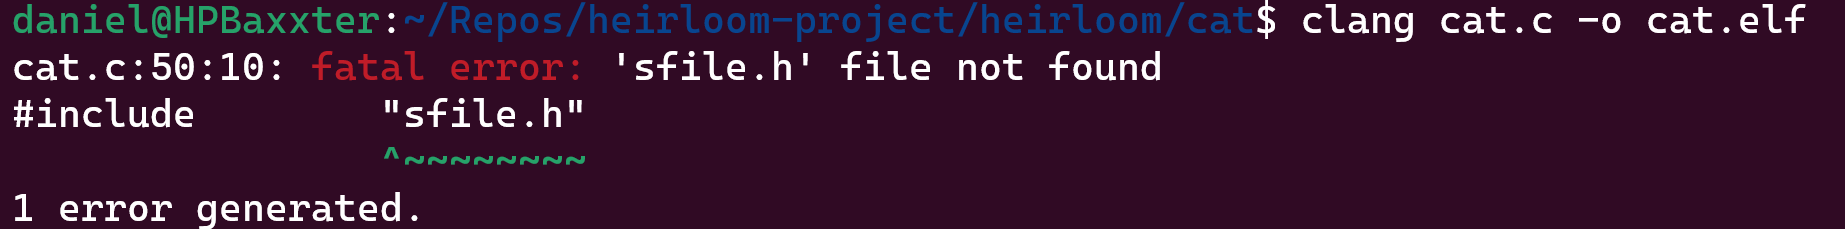
\includegraphics[scale=0.5]{Images/1_clang_cat.c.png}
	\caption{Fehlermeldung beim Versuch die Datei cat.c zu kompilieren}
	\label{clang_cat.c_fehler}
\end{figure}

In einem weiteren Versuch wurde versucht mit gcc zu kompilieren, allerdings führte dies zum selben Ergebnis.\par
Um dieses Projekt so zu kompilieren ist dies der falsche Ansatz gewesen.

\subsection[makefiles]
Für die Kompilation der Programm in diesem Repo hat Herr Ritter Makefiles angelegt.Das Programm make kann diese Makefiles verarbeiten.
Dazu muss diesem innerhalb des Makefiles mitgeteilt werden was das Programm ausführen soll, das ist das \textit{target}, und wie es dies ausführen soll, das ist die {textit{Regel}\cite{makefiles:2002}.
Dies wird genutzt um den Kompilationsprozess zu vereinfachen und somit können komplexere Kompilationsanweisungen einfacher ausgeführt werden.
Die Verlinkung werden in das Makefile geschrieben und somit muss nur noch der Befehl make genutzt werden.\par
Um die Programme des heirlomm-project zu installieren muss zunächst im Ordner heirloom der Befehl make und anschließend make install ausgeführt werden.
Beide Befehle sollten mit Superuserdo (sudo) ausgeführt werden.\par

\begin{lstlisting}
	sudo make
\end{lstlisting}

\begin{lstlisting}
	sudo make install 
\end{lstlisting}

Anschließend kann im Ordner des Programms cat der Befehl make verwendet werden.
Nun ist das Programm erfolgreich kompiliert und kann genutzt werden.
Das Programm kann mit folgendem Befehl ausgeführt werden.\par

\begin{lstlisting}
	./cat
\end{lstlisting}

Übergibt man nun eine Datei bei der Ausführung von cat wird der Inhalt der Datei in das Terminal geprintet.\par
Einige der Programm, wie zum Beispiel clock_settime, beinhalten veraltete nutzen veraltete Bibliotheken.
Im Falle von clock_settime wäre dies die Funktion stime\cite{stime:2023}.
Diese zu ersetzen ist allerdings nicht so einfach, wie im Tutorium festgestellt wurde.
Die einfache Ersetzung durch clock_settime funktioniert nicht und es sind noch weitere Änderung notwendig. \par

\section{Die Datei cat.1}
In dem Ordner des Programms cat befindet sich die Datei cat.1 .
Diese ist für die Erstellung der manpage des Programms cat geschrieben worden.
In dieser wird beschrieben wie das Programm ausgeführt werden kann.
Dazu werden alle Optionen und Übergabewerte beschrieben.\par


\section{Der Programmcode von cat.c}
In diesem Abschnitt wird der Code des Programms cat.c Zeile für Zeile durchgegangen, um nachzuvollziehen was dort geschieht. Dabei wird der Einleitende Kommentar von Gunnar Ritter übersprungen. Dort findet man Copyright Aussagen und Benutzungsrechte.

\subsection{Die Versionsabfrage von Gnuc und setzen der Flaggen}
Zu beginn, in den Zeilen 28 bis 34, des Codes findet man eine Versionsabfrage von \textit{GNUC} mittels einer if Kontrollstruktur. Diese soll feststellen welche Version des Compilers GNUC auf dem Gerät installiert oder ob dieser überhaupt installiert ist. Ist dieser in der Version höher oder gleich 3 \textbf{und} \textit{GNUC\_minor} höher oder gleich 4, wird der Variable USED über die \textit{Attribut Spezfikation} used zugewiesen. Dies geschieht auch wenn GNUC un der Version gleich 4 oder höher installiert ist, wenn die beiden voherigen Bedingungen nicht erfüllt sind.

\begin{lstlisting}
#define USED	__attribute__ ((used))
\end{lstlisting}

Sind diese Bedingungen nicht erfüllt, aber GNUC ist trotzdem installiert, wird der Variable USED das Attribut unused zugewiesen.

\begin{lstlisting}
#define USED	__attribute__ ((unused))
\end{lstlisting}

Ist GNUC überhaupt nicht installiert wird der Variable USED nichts zugewiesen. Sie wird aber initialisiert.

\begin{lstlisting}
#define USED
\end{lstlisting}

Im Anschluss an die if-Schleife, in der Zeile 35, wird der Variable USED ein statisches character array zugewiesen namens sccsid. Dies geschieht nur wenn der Variable USED auch das Attribut used zugewiesen wurde. In dieses Array werden die nach der Eingabe von cat im Terminal genutzten Flaggen aus der geschrieben.

\subsection{Eingebundene Bibliotheken}
Die Zeilen 37 bis 52 enthalten die für das Programm verwendeten Bibliotheksdateien.Diese enthalten die Funktionen die später im Code verwendet werden. Dabei soll hier jetzt nicht auf jede einzelne Bibliotheksdatei und deren Funktion eingegangen werden. Es finden sich allerdings auch "Standard-Bibliotheken" wir stdio.h oder stdlib.h wieder.

\subsection{Statische Variablen}
Der nächste Teil des Programmcode, von Zeile 54 bis 63, enthält mehrere Deklarationen von statischen Variablen. Diese behalten ihren zugewiesenen Wert über das ganze Programm hinweg, beziehungsweise diese  werden nicht neu initialisiert beim Aufruf eines Blocks in dem sich vorkommen. \par
Die erste initialisierte Variable ist errcnt. Diese soll die Fehlermeldungen beim ausführen des Programms zählen. Der dafür verwendete Datentyp ist unsigned, er kann also nur positive Werte speichern. Dies ist auch sinnvoll, da die Summe der Fehlermeldungen nicht negativ sein kann. \pari
Weiterhin werden einige Variablen für verwendete Flaggen initialisiert, eine für den Programmname, eine Nutzerdefinierte Struktur und ein integer namens multibyte.\par

\subsection{Funktionen}
Ab der Zeile 65 beginnen die Funktionsbeschreibungen die in dem Programmcode von cat genutzt werden.\par
Die erste Funktion nennt sich srealloc und ist eine Speicher neu Belegung. Mit dem Befehl realloc wird eine Speicher neu Belegung durchgeführt.
Dabei wird die Größe des benötigten Speichers mit übergeben.
Wenn nicht genügend Speicher zur Verfügung steht ist der Returnvalue der Funktion realloc gleich NULL.
Ist dies der Fall, ist die Bedingung in der Funktion srealloc erfüllt und es wird eine Fehlermeldung in das Terminal geprintet.
In dieser Fehlermeldung steht das kein Speicher zur Verfügung steht und das Programm wir über den Exit-Befehl beendet.
Dabei wird der Exitcode 077 an das Betriebssystem zurückgegeben.
Der Code 077 ist eine Zahl mit oktaler Basis und steht für die Zahl 63, in dezimale Schreibweise.\par
Die nächste Funktion nennt sich usage.
Mit dieser Funktion kann die richtige Verwendung des Programms cat ausgegeben werden.
Wird diese Funktion ausgeführt beendet diese nach der Ausgabe das Programm.\par
Als nächstes folgt die Funktion writerr.
Diese Funktion dient dazu Fehler bei der Ausgabe darzustellen.
Dies geschieht nur wenn die Option -s bei der Ausführung nicht genutzt wird.
Dies wird über eine If-Verknüpfung abgefragt.
Die Option -s ist die silent Option.
Diese verhindert das einige Fehlermeldungen nicht ins Terminal geprintet werden sollen.
Ist die Option nicht gesetzt gibt die Funktion eine Fehlermeldung aus, in der der Programmname und die Anzahl der geschriebenen Zeichen im Verhältnis zu den Gesamtzeichen, sowie eine Fehlercode mithilfe von der Funktion strerror.
Außerhalb der If-Verknüpfung befindet sich noch eine weitere Operation.
Bei dieser wird der errorcount bitweise mit der Zahl 4 verknüpft.
Dies geschieht immer beim Aufruf der Funktion unabhängig von der Option -s.\par
Als letzte Funktion folgt noch die copy Funktion, die auch die längste der enthaltenden Funktionen ist.
Diese enthält die eigentlich Programmfunktion, also das kopieren des Inhalts der Datei oder Eingabe.
Innerhalb der Funktion befinden sich mehrere Fehlerbehandlung, die wieder in Abhängigkeit der -s Option ausgegeben werden.
Darunter finden sich Fehler die zum Beispiel das öffnen der übergebenen Datei betreffen oder auch das fehlerhafte Lesen der Datei betreffen.
Ebenfalls gibt es eine Fehlermeldung wenn die \textit{input-Datei} die selbe ist wie die \textit{outtput-Datei}.
Innerhalb der Funktion werden außerdem verschiedene übergebene Optionen berücksichtigt.
In Abhängigkeit dieser wird der Inhalt der übergenen Datei bearbeitet.
Ebenfalls wird innerhalb der Funktion das Zielsystem Linux berücksichtigt.

\begin{lstlising}
	#ifdef __linux__
	....
	#endif /* __linux */
\end{lstlisting}

Dort wird mit einer Präprozessor Anweisung überprüft ob das Zielsystem auf Linux basiert.
Wird das Programm auf einem Linux basierten System kompiliert werden diese Anweisungen mit ausgeführt.
In diesem Abschnitt wird die Dateiübertragung für Linuxsysteme überprüft.

\subsection{main}
Zum beginn der main werden zunächst zwei Variablen initalisiert.\par
Anschließen folgt eine Präprozessoranweisung, zur überprüfung der gnu c library.
Diese stellt einige für Unixsysteme vorhandene C-Funktionen zur Verfügung.
In diesem Fall wird die Variable POSIXLY_CORRECT auf eeins gesetzt.
Dies dient dazu einige Funktionen im Programm dem POSIX-Standard anzupassen.\par
Anschließend wird der Variablen progname dem wert des argument value null zugewiesen.
Mit dem folgendem Befehl setlocale wird das Betriebsystem aufgefordert die lokale Sprache und Einstellungen des Systems dem Programm zu übergeben.
Damit können die Zeichen die das System verwendet auch im Programm genutzt werden.
In dem folgendem Befehl wird überprüft ob das System Multibyte-Zeichen unterstützt. 
Ist dies der Fall wird der Wert von multibyte auf einen Wert größer als eins gesetzt.
Ist dies nicht der Fall, und das System verwendet nur ein Byte pro Zeichenkette, wird dort eine 1 gesetzt.\par
Das Programm überprüft nun mit Befehl getopt, welche Optionen dem Programm übergeben wurden. 
Ist eine der mögliche Optionen übergeben worden wird die dafür initialisierte Variable auf den Wert 1 gesetzt.
Wird die die Option --help genutzt. Wird die Funktion usage aufgerufen und die Verwendung des Programms und dessen Optionen wird ins Terminal geprintet.\par
Nun wir der Nutzerdefinierten Struktur op über die Funktion ob_alloc ein Datenstruktur zugewiesen.
Dieser hängt davon ab welche Flaggen genutzt werden.\par
Anschließend erfolgt eine weitere Fehlerbehandlung.
Dort wird der Dateideskriptor zum Standard out überprüft.
Kann dieser nicht festgestellt werden gibt die Funktion den Wert 1 zurück.
Dies bedeutet das Fehler aufgetreten ist und das Programm wird mit der Fehlermeldung und dem Exitcode 1 beendet.\par
Der nächste Code-Abschnitt überprüft die Anzahl der übergebenen Optionen.
Dies wird mit einer if-Abfrage umgesetzt.
Dort wird überprüft ob die Anzahl der übergebenen Optionen ungleich dem argument count ist.
Ist dies der Fall folgt eine while-Schleife, in der Funktion copy solange aufgerufen wird bis der option index kleiner dem Wert argument count ist.
Da dieser Teil solange aufgerufen wird bis beide Werte gleich sind, endet dort die while-Schleife.
Anschließend zu der if-Abfrage folgt die else-Behandlung.
Dort wird einmalig die Funktion copy aufgerufen.\par
Mit dem folgenden Aufruf der Funktion ob_free wird vermutlich der Speicher den der Zeiger op verwendet wieder freigegeben.
Nun wird noch der Dateideskriptor zum Standard output geschlossen.
Ist dies erfolgreich gibt die Funktion close den Wert 0 zurück.
Im Fehlerfall ist der Wert -1 und somit kleiner als 0.
Dies führt dazu das, im Falle der nicht gesetzten -s Option, eine Fehlermeldung in das Terminal geprintet wird.Ebenfalls wird wieder der Errorcount bitweise um 4 erhöht.\par
Zum Ende des Programms wird noch der returnvalue zurückgegeben. 
Dieser entspricht dem im Programm vorgekommen error count, also der Anzahl der Fehler.
Tritt kein Fehler auf ist dieser 0.\par
